\documentclass[tikz,border=8pt]{standalone}
\usepackage[T1]{fontenc}
\usepackage{helvet}
\renewcommand{\familydefault}{\sfdefault}
\usetikzlibrary{arrows.meta, backgrounds}

\definecolor{phasefill}{HTML}{F4F7FB}
\definecolor{phaseborder}{HTML}{9AA7B4}
\definecolor{datafill}{HTML}{FFF4D6}
\definecolor{databorder}{HTML}{D9A441}
\definecolor{llmfill}{HTML}{DFF7F3}
\definecolor{llmborder}{HTML}{1BA99C}
\definecolor{toolfill}{HTML}{E9EDFF}
\definecolor{toolborder}{HTML}{6979C9}
\definecolor{outfill}{HTML}{E7F6E7}
\definecolor{outborder}{HTML}{4FA64F}
\definecolor{darkline}{HTML}{333333}

\tikzset{
  panel/.style={
    rectangle,
    rounded corners=10pt,
    fill=phasefill,
    draw=phaseborder,
    line width=1pt
  },
  box/.style={
    rectangle,
    rounded corners=5pt,
    align=center,
    draw=darkline,
    line width=0.8pt,
    minimum height=0.9cm,
    font=\small
  },
  input/.style={
    box,
    fill=white,
    minimum width=2.3cm
  },
  data/.style={
    box,
    fill=datafill,
    draw=databorder,
    minimum width=3.2cm
  },
  llm/.style={
    box,
    fill=llmfill,
    draw=llmborder,
    minimum width=3.0cm,
    font=\small\bfseries
  },
  output/.style={
    box,
    fill=outfill,
    draw=outborder,
    minimum width=3.0cm
  },
  context/.style={
    box,
    fill=white,
    minimum width=3.4cm
  },
  tool/.style={
    box,
    fill=toolfill,
    draw=toolborder,
    dashed,
    minimum width=1.75cm,
    font=\scriptsize
  },
  flow/.style={
    -{Latex[length=2.2mm]},
    line width=0.85pt,
    draw=darkline
  },
  phase-title/.style={
    font=\small\bfseries,
    align=center
  }
}

\begin{document}
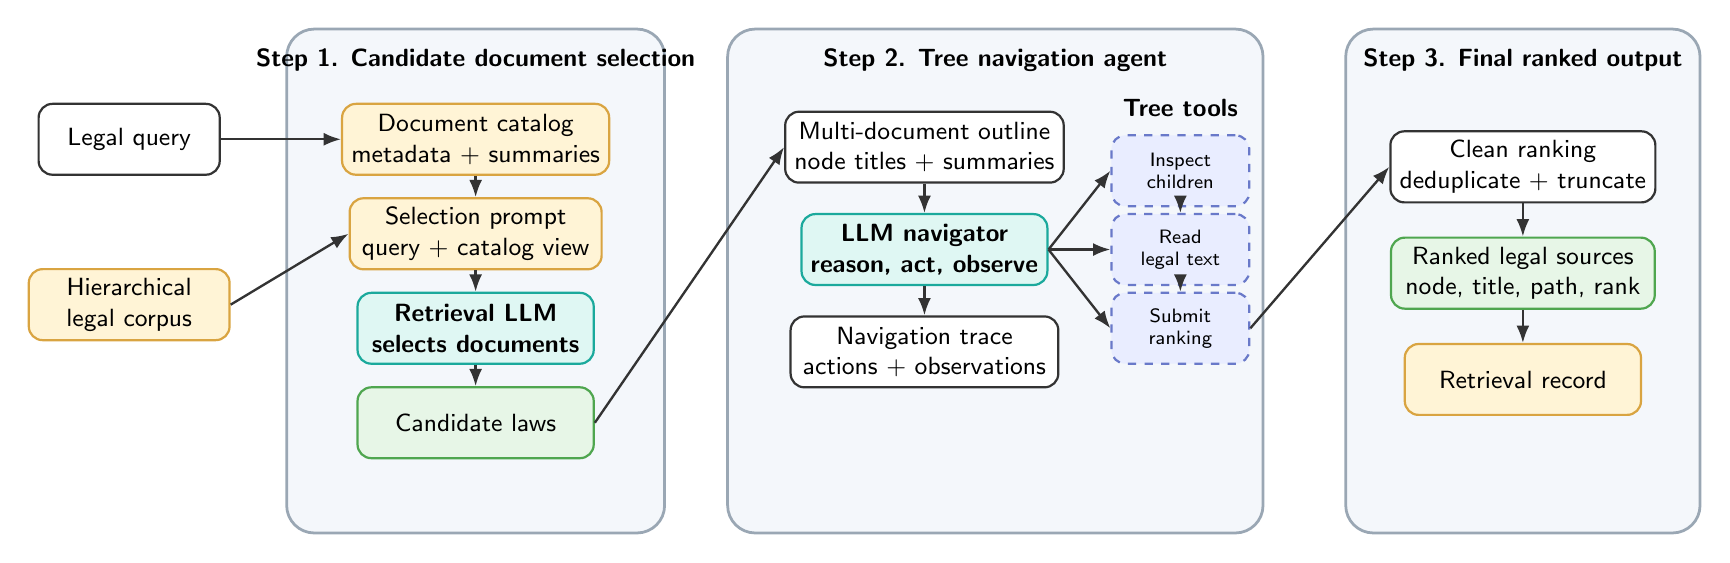
\begin{tikzpicture}

% Fixed panels. These are deliberately explicit so the layout is stable.
\begin{pgfonlayer}{background}
  \node[panel, minimum width=4.8cm, minimum height=6.4cm] at (4.4, 3.55) {};
  \node[panel, minimum width=6.8cm, minimum height=6.4cm] at (11.0, 3.55) {};
  \node[panel, minimum width=4.5cm, minimum height=6.4cm] at (17.7, 3.55) {};
\end{pgfonlayer}

% Inputs.
\node[input] (query) at (0.0, 5.35) {Legal query};
\node[data, minimum width=2.55cm] (corpus) at (0.0, 3.25) {Hierarchical\\legal corpus};

% Step 1.
\node[phase-title] at (4.4, 6.35) {Step 1. Candidate document selection};
\node[data] (catalog) at (4.4, 5.35) {Document catalog\\metadata + summaries};
\node[data] (prompt) at (4.4, 4.15) {Selection prompt\\query + catalog view};
\node[llm] (selector) at (4.4, 2.95) {Retrieval LLM\\selects documents};
\node[output] (laws) at (4.4, 1.75) {Candidate laws};

% Step 2.
\node[phase-title] at (11.0, 6.35) {Step 2. Tree navigation agent};
\node[context] (outline) at (10.1, 5.25) {Multi-document outline\\node titles + summaries};
\node[llm] (navigator) at (10.1, 3.95) {LLM navigator\\reason, act, observe};
\node[context] (trace) at (10.1, 2.65) {Navigation trace\\actions + observations};

\node[phase-title] at (13.35, 5.75) {Tree tools};
\node[tool] (inspect) at (13.35, 4.95) {Inspect\\children};
\node[tool] (read) at (13.35, 3.95) {Read\\legal text};
\node[tool] (submit) at (13.35, 2.95) {Submit\\ranking};

% Step 3.
\node[phase-title] at (17.7, 6.35) {Step 3. Final ranked output};
\node[context, minimum width=3.35cm] (clean) at (17.7, 5.0) {Clean ranking\\deduplicate + truncate};
\node[output, minimum width=3.35cm] (ranked) at (17.7, 3.65) {Ranked legal sources\\node, title, path, rank};
\node[data, minimum width=3.0cm] (record) at (17.7, 2.3) {Retrieval record};

% Main flows.
\draw[flow] (query.east) -- (catalog.west);
\draw[flow] (corpus.east) -- (prompt.west);
\draw[flow] (catalog) -- (prompt);
\draw[flow] (prompt) -- (selector);
\draw[flow] (selector) -- (laws);

\draw[flow] (laws.east) -- (outline.west);
\draw[flow] (outline) -- (navigator);
\draw[flow] (navigator) -- (trace);

% Tool interaction. Use short, straight arrows to avoid visual tangles.
\draw[flow] (navigator.east) -- (inspect.west);
\draw[flow] (navigator.east) -- (read.west);
\draw[flow] (navigator.east) -- (submit.west);
\draw[flow] (inspect.south) -- (read.north);
\draw[flow] (read.south) -- (submit.north);

\draw[flow] (submit.east) -- (clean.west);
\draw[flow] (clean) -- (ranked);
\draw[flow] (ranked) -- (record);

\end{tikzpicture}
\end{document}
